% -*-latex-*-
%
% Senior Project Final Report
%

\documentclass[a4paper,12pt]{article}
\usepackage[noend]{algorithmic}
\usepackage[section]{algorithm}
\usepackage{latexsym}
\usepackage{amsmath, amstext, amsthm, graphics}
\title{Graph Partitioning by Vertex Separators}
\author{Eray \"Ozkural}
\date{\today}
\begin{document}
\maketitle
\begin{abstract}
Graph partitioning is a cardinal problem that has extensive
applications in various areas such
as task scheduling, VLSI design, and scientific computing. 
First we give an introduction on partitioning, and describe the
problem. Then we study it by examining the leading studies,
explicating the multilevel algorithms, analyzing the VFM algorithm, and
pointing out the problem's relations with search problems.
We also introduce new techniques for matching vertices and
an improved version of VFM. We then describe our software library that
we have developed and justify its design.
We conclude that the multilevel methods which we have employed in our
software are the theoretically strongest methods, and that the
algorithmic components of our software are all well adjusted to
finding good vertex separators in an efficient manner.

\end{abstract}

\tableofcontents
\listoffigures
%\listoftables
\pagebreak

\section{Introduction}

Graph partitioning is a cardinal problem that has extensive
applications in various areas. The problem is concerned with
splitting a graph into $k$ parts which are approximately equivalent
in size. The partition is separated by a set of either \textsl{edges}
or \textsl{vertices}. There are many parameters and criterion for the
quality of the partition. For instance, a specific application may
require that a two way partition is separated by a minimum number of
edges. As Liu \cite{liu} notes, the fundamental importance of the
problem is due to its strong connection to the divide-and-conquer
paradigm. Many search problems with detailed structure and global
goals lend themselves to graceful modeling with the partitioning problem such
as task scheduling, VLSI design, and scientific computing. 

\subsection{Report Overview}

This report, succeeding a lengthy introduction about graph
partitioning, describes the main problem of the project in which we
provide a short section on preliminaries for graph algorithms, and
then give a moderately formal definition for the specific problems we
are interested in. Thereafter, we confront the graph partitioning  by
vertex separator problem in a  theoretical light by examining the
leading studies, explicating the details of multilevel algorithms,
analyzing the favored VFM algorithm, pointing out to the problem's
 relation with
general search methods, and introducing new techniques for matching
vertices and an improved version of VFM. Having left the theoretical
sphere, we then describe the software we have contrived by looking at
its algorithmic components, the choice of implementation platform,
then a brief overview and performance discussion. The report finishes
with a statement of our conclusions and directions for future work.

In the following subsections of introduction, we will
introduce some of the common applications, then the methods used for solution,
and following that our goals together with the course of work we have
accomplished.

\subsection{Application Domains}

Not surprisingly, the first problems that were recognized to be
effectively modeled by graph partitioning come from the realm of
computers and engineering. Kernighan and Lin describe the problems of
placement of electronic components, and optimizing paging properties
of programs as immediate examples \cite{kl}. Since then, graph
partitioning has proven to be a versatile tool in VLSI design and
many software problems. Following are examples to
common applications of graph partitioning.
\begin{itemize}
\item The problem of task scheduling for parallel computing
suits beautifully to graph partitioning problem. Since one would wish to
reduce the expensive communication between tasks, she can model the
tasks as vertices and the communication volumes as edges of an
ordinary graph. A partition of the graph into the number of processors
which minimize the total communication volume would then give
an exact solution to her needs.
\item The solution of sparse symmetric matrices, for instance
in linear programming, is best described as a graph partitioning
problem in which the $n$ vertices of the graph correspond to the n
columns of the matrix and the edges represent the non-zero elements of
the matrix.\cite{bend} Although there are algorithms which operate
directly on matrices, the graph partitioning based algorithms have
been shown to be more powerful.\cite{gupta1} \footnote{Note that such
a matrix and a graph are numerically identical structures, however
the graph theoretic approach yields more elegant and effective
results.}
\end{itemize}
\subsection{A Tour of Methods}
Because of its spectacular generality, several methods to solve the
partitioning problem have been developed for more than three
decades. Since the problem is known to be NP-complete, any solution
has to be based on heuristics. Currently, there are various heuristic
methods which give partitions of high quality within reasonable
time-space bounds.\cite{gupta1} 

One of the first breakthroughs in graph partitioning problem is due
to Kernighan and Lin \cite{kl} in their now classical paper. To date,
heuristic procedures usually employ a form of their approach. In that
paper, they rule a number of false heuristics out.\footnote{They give a
measure of how big the search space is, they state that for a 32x32
matrix the chance of a random trial to hit the optimal peak is about
$10^{-7}$.}

We should first distinguish between two families of algorithms:
\begin{description}
\item{\textbf{Single-Level Algorithms}} These algorithms operate on
the graph as a whole. That is they do not derive an equivalent
structure instead of the graph (or matrix). The terms in  their
formulation usually correspond to sets or elements of vertices (edges) of the
graph. They work by finding an initial partition and then improving
it according to a heuristic.
\item{\textbf{Multi-Level Algorithms}} Multilevel algorithms first
reduce the size of the graph by collapsing vertices (and edges as
accordingly), and then partition this condense representation of the
fine graph. The next step is to project the partition of the coarse
graph to the original one. The more effective of these
algorithms refine the algorithms at each level while projecting using
a heuristic. All three steps mentioned can be performed in differing
manners, thus making the overall algorithms distinct. A survey and
evaluation of multilevel methods is available in \cite{kumar}. 
\end{description}

We shall now give a broad classification of algorithms, in another
section we will dwell on the type of algorithms to our special interest.
\begin{description}
\item{\textbf{Spectral Partitioning Algorithms}} These algorithms
employ computation of the eigenvector corresponding to the second
smallest eigenvalue. Although they give good quality partitions, they
are not very time efficient. The multilevel spectral bisection
algorithm is faster, however they are not comparable to multilevel
graph partitioning algorithms. \cite{kumar}
\item{\textbf{Geometric Partitioning Algorithms}} This class of algorithms
makes use of geometric information of vertices, and work quite fast
although the randomized nature of the algorithms do not permit
quality as high as SP. In addition to this, the frequent unavailability of
geometric information make these algorithms less attractive. \cite{kumar}
\item{\textbf{Minimum Degree Ordering:}} There are simple greedy
algorithms which try to eliminate the vertex with the minimum degree.
These algorithms work quite fast and are capable of giving good
quality partitions. Because of the speed, they are
popular. Unfortunately, they can deviate far from the
optimal\cite{bend}. They have advanced variants such as
MMD.\footnote{Multiple Minimum Degree.}
\item{\textbf{Nested Dissection Algorithms}} The algorithms that
recursively obtain a partition of the graph are called nested
dissection algorithms.\cite{liu} \cite{bend} ND algorithms, until
recent, were inferior to minimum degree algorithms. One advantage
of them is that they are more explicable by theoretical study.
\item{\textbf{Gain Heuristic Algorithms}} First described by Kernighan
and Lin\cite{kl}, and improved by Fiduccia and Mattheyses\cite{fm} a
popular heuristic method is determining all simple operations on the
partition (such as moving or interchanging a single vertex) and
performing the one which improves the partition most. This local
strategy has turned out to be useful and efficient
implementations of it have been devised.\cite{kumar} \cite{bend} \cite{gupta1}
\item{\textbf{Vertex Cover Algorithms}} Liu describes a single-level
iterative method which operates on a set of vertices instead of single
vertices as in gain heuristic algorithms.\cite{liu} It has been
understood that his algorithm finds a vertex cover of the vertices in
the separator and their neighbors in a partition.\cite{bend}
\footnote{This gives
rise to better theoretical treatment of the algorithm, and of course
better conceiving the limits of the approach}. A generalization of the
algorithm then becomes finding the minimum weighted vertex cover.
\end{description}

At this point, it should be mentioned that no graph partitioning
package is comprised of merely one of the algorithm classes
introduced. Basically, the algorithms are applied when they are most
useful since a host of theoretical attributes and empirical profile
about them are known. For instance, at one point the algorithms can
abandon doing nested dissection and commence with minimum
degree.\cite{bend} Naturally, the co-operating algorithms will have to be
modified and good metrics and control systems for switching execution
will have to be devised.

The reader is referred to \cite{kumar}, \cite{bend} for a survey of
partitioning algorithms.

\subsection{Methodology and Goals}

The objective of this project was initially to be content with a
decent node separator improvement that can get along with the
\textsc{Patoh} package developed by \"{U}mit \c{C}ataly\"urek of Bilkent
University. However, there have been problems and the need to
alter our course a bit has occured.

\subsubsection{Problems Encountered}
We have faced two major problems while trying to realize our work
on implementing Liu's iterative improvement algorithm
\begin{itemize}
\item The complexity of the \textsc{Patoh} system made it quite
difficult to read between the lines and accomplishing clean
coding. While a small peak of C code was developed, it had taken
longer than we had thought, and it was abandoned for other reasons.
\item When it was realized that no real improvement over Liu's
algorithm in the hypergraph domain was possible, we decided to change
track. Liu's algorithm effectively computes a vertex cover, and there
is not much out of a vertex cover.
\end{itemize}

\subsubsection{A New Look}
Thereafter, we began looking into the vertex separator problem on its
own. We left integration with \textsc{Patoh} to a later period, and
focused on the essentials of vertex separators and the
state-of-the-art in the field.

\subsubsection{Goals}
We would then embark on the vertex separators. We would certainly have
to answer a few questions.
\begin{itemize}
\item What is the most effective and rigorous theory around?
\item Could any theoretical advancements be made at it?
\item How can we implement a graph partitioning program from scratch?
\end{itemize}

The questions are not trivial to find out and it has been our task to
realize their answers.

\section{Problem Description and Background}

In this section we will provide a formal description and some
background for the problem.

\subsection{Preliminaries}

\newtheorem{dfn}{Definition}
\begin{dfn}
\textbf{Graph:}
A graph $G=(V,E)$
is an ordered pair of a set of \textsl{vertices} $V$ and
a set of \textsl{edges} $E$ where
\begin{equation}
\forall u,v {(u,v) \in E} \rightarrow {u \in V \wedge v \in V}
\end{equation}
In edge $(u,v)$ u is adjacent to v.Edge $(u,v)$ is incident to vertex $s$ if $u=s \vee v=s$.
\end{dfn}


Since we will be completely involved with graphs, it should be clear that when we refer
to $V$ or $E$ sets, we also refer to a graph $G=(V,E)$. For a simple graph, see figure \ref{fig:1}.

In order to be able to describe algorithms in concise form there are
some standard functions \footnote{Which surely correspond to certain
data structures and procedures.}. Without hesitation we describe some
of them.

\begin{dfn}
\textbf{Useful Functions:}
Let $X,Y$ be sets of vertices of $G$, and $x \in V$.
\begin{itemize}
\item $Adj_G(x)$ refers to the set of vertices of $G$ which are adjacent to x.
\item $Adj_G(X) = \{ u | x \in X \wedge u \in Adj_G(x) \wedge u \notin X\}$
\item $Adj_G(x, Y) = Adj_G(x) \cup Y$
\item $Adj_G(X, Y) = Adj_G(X) \cup Y$
\end{itemize}
We shall drop subscripts whenever it is clear from the context.
\end{dfn}


\begin{figure}
\begin{center}
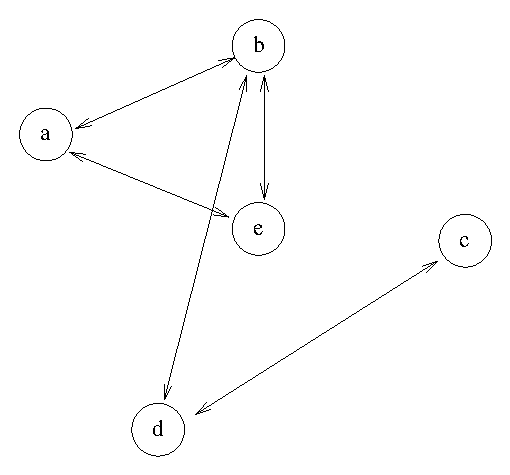
\includegraphics{simple_graph.eps}
\caption{A simple graph with vertices ${a,b,c,d,e}$ and a few edges}
\label{fig:1}
\end{center}
\end{figure}

\begin{dfn}
\textbf{Path:} A path is a sequence $S=<v_1,\dots,v_k>$ of vertices
such that $\forall i,i+1 \in S, {(v_i,v_{i+1}) \in E}$.
\end{dfn}

\begin{dfn}
\textbf{Connected Graph:} A complete graph is graph in which from any
vertex there is a path to every other vertex.
\end{dfn}

\begin{dfn}
\textbf{Connected Component:} A subgraph $G'=(V',E')$ such that
G' is connected and there is no path between $G-G'$ and $G'$.
\end{dfn}

\begin{dfn}
\textbf{Matching:} A matching $m$ in $G$ is a set of edges which do
not share any vertex. A maximal matching is a matching that cannot be
enlarged by addition of any edge $(u,v) \in G-M$.
\end{dfn}

\begin{dfn}
\textbf{Vertex Cover:} Vertex cover is a set of vertices $C$ such that
every edge in $E$ is incident to a vertex in $C$. It should be obvious
that a vertex cover is equivalent to a maximal matching.
\end{dfn}

\subsection{Problem Description}

\begin{dfn}
\textbf{K-way Graph Partitioning Problem:} The k-way partition of a
connected graph is defined as follows. Let a connected graph $G=(V,E)$
where $|V|=n$
be partitioned into subsets $V_1,V_2,\dots,V_k$ such that for all
$1\le i \le j \le k$, 
$ V_i \cap V_j = \emptyset $
and
$|V_i| \cong n/k $ and $ \bigcup_i{V_i=V} $
where edge cut $E_c = \{(u,v) | (u,v) \in E \wedge
\exists i,j (i \ne j \wedge u \in V_i \wedge v \in V_j) \}$ .
$|E_c|$ is minimal.
\end{dfn}

The formal definition also introduces $E_c$ the edge cut. Indeed, we
can define graph partitioning by edge separator in other words:
\begin{dfn}
\textbf{K-way Graph Partitioning Problem (alt):}
Removal of the edge separator $E_c$ partitions the connected graph $G$
into $k$ roughly equal connected components.
\end{dfn}

As previously stated, partitioning of a graph by edge separator is
distinct from partitioning of a graph by vertex separator.
\begin{dfn}
\textbf{K-way Graph Partitioning by Vertex Separator Problem:} The k-way partition of a
connected graph by vertex separator is defined as follows. Let a
connected graph $G=(V,E)$
where $|V|=n$
be partitioned into subsets $V_1,V_2,\dots,V_k$ and $V_s$ such that for all
$1\le i \le j \le k$, 
$ V_i \cap V_j = \emptyset $
and
$|V_i| \cong \frac{n-|V_s|}{k} $ and $ \bigcup_i{V_i=V-V_s} $
and $\forall u,v (u \in V_i \wedge v \in V_j) \rightarrow (u,v) \notin E$   
$|V_s|$ is minimal.
%where vertex separator $V_s = \{u | u \in V \wedge
%\forall 1\le i\le k (u \notin V_i   ) \}$ .
\end{dfn}

We will denote $V_s$ with $S$ in the rest of the paper, and in 2-way
graph partitioning problem by vertex separator, which is also known as
graph bisection by vertex(node) separator problem, $V_1$ and $V_2$
will be denoted with $X$ and $Y$ respectively.

An immediate extension to these problems is the addition of vertex
and edge weights. We will denote vertex weights by $w(x)$ and edge
weights by $w(u,v)$. In general, if there are no weights in the
graph these quantities may be safely assumed to be $1$ for all
existent vertices and edges. Note that addition of the weight notion
changes the problem description in that:
\begin{itemize}
\item In the edge separator problem we minimize $\sum_{(u,v) \in
E_c}{w(u,v)}$ and consider the total vertex weight of partitions for the balance
constraint.
\item In the vertex separator problem we minimize $\sum_{u \in
S}{w(u)}$ and consider the total vertex weight of partitions for the
balance constraint.
\end{itemize}

\section{Theoretical Exposition}

We will now explore the theoretical details of the graph
partitioning by vertex separator problem. First, we will see
what algorithms are of exclusive importance to us, then we
will inspect those algorithms and their components. We will
also scrutinize theoretical relations and suggest improvements.

\subsection{Vertex Separator Algorithms}

The partitioning by vertex separators and edge separators
seem to be similar and they indeed share a lot of the
characteristics, concepts and processes. Nevertheless,
 their solutions are not identical, despite the obvious
clues. Hendrickson and Rothberg report that first finding
an edge cut and then converting it to a node separator is
prone to failure.\cite{bend} It is shown that a good edge
separator can give rise to low quality node separator.

Since our subject is vertex separators, we wish to
investigate the theory behind the algorithms that yield the best
results. Although we are acquainted with a number of studies on
graph partitioning algorithms, merely two of them concentrate
on vertex separators. 
\cite{liu} \cite{bend} In any case, the other works remain relevant in
at least the following respects:
\begin{itemize}
\item Multilevel algorithms show correlation in that they are imploded
and exploded to grab a global view of the graph.
\item The gain improvement heuristics are similar in that they move
single vertices complying with a balance constraint and trying to
get at a global goal. This in the worst case means that the algorithms use
similar techniques.
\end{itemize}

The main differences of edge and vertex separators may be
summarized as follows:
\begin{itemize}
\item In the formulation of graph partitioning by vertex separator, we
are usually not concerned with edge weights at all.\footnote{Of course
it may be the case that we wish to consider edge weights as well.}
\item In the gain heuristics computation, it is easier to manage
information about the individual gains of vertices since all vertices
we will consider moving are trapped in $S$.
\item The initial partition of a vertex separator need not be small,
since a tiny initial partition can inhibit refinement.\cite{gupta1}
\item Choosing a node separator from a minimum edge separator
has fatal flaws. A good edge separator is not necessarily a good node
separator. Figure \ref{fig:2} gives a straightforward example.
\end{itemize}

\begin{figure}
\begin{center}
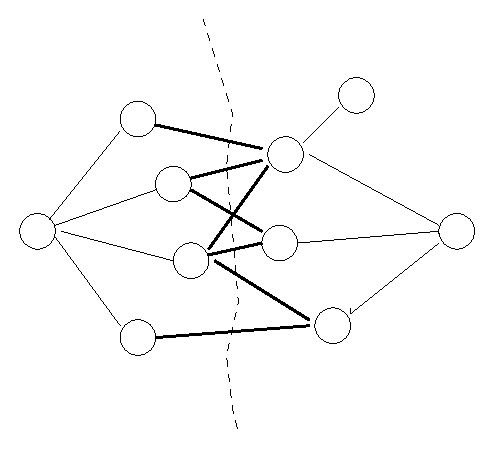
\includegraphics{edgesep_nodesep.eps}
\caption{The edge separator (bold edges) will not produce a good vertex separator}
\label{fig:2}
\end{center}
\end{figure}


The experimental work conducted in \cite{kumar},\cite{bend} and
\cite{gupta1} show that the multilevel graph partitioning algorithms
are superior to other methods including MMD, and MSB\footnote{
Multilevel spectral bisection.}.Hence we shall expound the better class
of algorithms, paying attention to the properties of vertex separators
that we have remarked.


\subsection{Multilevel Graph Partitioning Algorithms}

In this section we shall present a multilevel graph bisection
algorithm. In general, we may hope to generalize a bisection
procedure to a k-way partitioning procedure as in \cite{kl}.

A multilevel graph bisection algorithm consists of three phases.\cite{kumar}
\begin{description}
\item \textbf{Coarsening Phase} Starting with the original graph $G_0$
this phase generates a sequence $L=<G_0,G_1,\dots,G_m>$ such that
$|V_0| > |V_1| > \dots >|V_m|$. At each step the coarsening algorithm
reduces the number of vertices of a graph. There are various methods
for the procedure, however  the basic principle is that a number of
vertices are grouped to form a vertex of the coarser graph.

Let $V_i^v$ be the set of vertices of $G_i$ combine to form vertex v
of $G_{i+1}$. In order to maintain quality of bisection the
information of vertex weights must be accumulate. The weight of vertex
v, which we shall call a \textsl{supernode}, equals to the sum of
weights of vertices in $V_i^v$ and the weights of edges may computed
according to the same summation principle. However, we do not compute
edge weights since we don't require them for vertex separators.
\begin{equation}
	v=V_i^v, w(v) = \sum_{x \in V_i^v}{w(x)}
\end{equation}

The methods differ in the way vertices to collapse are selected. Among
the popular methods are collapsing matched vertices in a matching of
the graph, an choosing vertices which are highly connected. When
matchings are used, we effectively crunch pairs of vertices into
single vertices. Since we wish to eliminate as many vertices as
possible, we compute a maximal matching of the graph. Generally,
maximum matchings are not computed because of their greater running
time complexity.

Coarsening procedure preserves a number of graph properties including
planarity and connectivity. It may be thought that the more essential
information a compressed graph preserves, the better our algorithm
will work.

A coarsening procedure has some parameters which can be altered:
\begin{itemize}
\item The maximum number of vertices in $G_m$
\item The procedure that selects the vertices to collapse at each
level
\end{itemize}

As long as the former parameter is kept low enough,
it does not make a significant change in the result. The latter
parameter, however, may have influence on the running of the
algorithm. It is possible to select vertices so that we can approach
the objective earlier. In our design, we considered random matching (RM),
heavy edge matching(HEM) and a new matching that we
introduce. However, the experimental data suggests that the
improvement in quality is often marginal.\footnote{At least in the
work of other researchers.} Some matching schemes are
\begin{description}
\item{\textbf{Random Matching}} An efficient matching can be contrived by
means of random visiting of vertices. We iteratively match unmatched
vertices with random adjacent vertices until a random matching is
obtained. The algorithm runs in $O(E)$ time.
\item{\textbf{Heavy Edge Matching}} This is a variation of RM which, in a
random vertex visit order, picks adjacent edges with most
weight. Since it absorbs heavy edges, it helps find a good edge
separator. However, because of the reasons explained previously, we do
not choose an algorithm that tries to find a good edge separator.
\item{\textbf{Triangle Matching}} These methods select more than 2 vertices
for collapsing, and they seem to be more efficient with small
compromise in quality \cite{gupta1}.
\item{\textbf{Other Metrics}} It seems plausible that more
sophisticated measures than the most trivial might be used for
selecting which vertices to collapse. Graph compression is one of
these ways, described in \cite{bend}. We think that a carefully
designed metric can help improve the quality of partitions.
\end{description}

\item \textbf{Partitioning Phase} In $G_m$ it is much easier to
compute a good partition $P_m$, since the size of the coarsest graph is
reasonable. \footnote{We set the threshold to under 100 so time for finding the
initial separator is insignificant.} Hence, we can allow for randomized
algorithms which pick the best partition out of a couple of
runs. Nevertheless, heuristics even at this level are of
utility. It turns out that using other methods such as MSB, or
geometric partitioning does not give us advantage even at this small
scale\cite{kumar}. Gupta \cite{gupta1} argues that no initial
partitioning is necessary since partitioning is the bottom up
equivalent of coarsening, and goes to some lengths for the sake of
argument. His package coarsens the graph until $k$ vertices are
obtained; corresponding to $k$ partitions. On the contrary,  the idea
of applying the same algorithm at all scales does not seem that clear
to us. It is doubtable whether $k$ vertices should represent $k$
partitions. The crucial point for us is to find an initial vertex
separator directly, whose size might be big. The algorithm we employ
gives us such an initial partition, described in algorithm \ref{alg:bisect}.

\begin{algorithm}
\caption{$\textsc{Levelized-Bisection}(G)$} \begin{algorithmic}[1]
\label{alg:bisect}
\STATE{compute a pseudo diameter of $G$}
\STATE{levelize $G$ from one extreme of the diameter}
\STATE{take the level which maximizes balance as the vertex separator }
\end{algorithmic}\end{algorithm}

Note that the algorithm is similar to the graph growing algorithms
\footnote{ These algorithms start from a vertex and grow around it a
region in breadth-first fashion  until half of the vertices are
included.} used for finding edge separators. In \cite{bend}, it is
claimed that any partitioning algorithm may be used, but the evidence
from other work suggest that the algorithms are not totally
insensitive to the initial partition.

\item \textbf{Uncoarsening Phase} The uncoarsening phase is
responsible for projecting back the partition $P_m$ to the original
graph. This is performed in successive projections to finer graphs in
the sequence of
$G_{m-1},\dots,G_0$ until the partition on the original graph is
obtained.
Computing $P_{i}$ from $P_{i+1}$ is straightforward: $\forall u \in V_i^v
P_i[u] = P_{i+1}[v]$ \cite{gupta1}. We simply map the partition of a
collapsed vertex to its constituent vertices during a projection. In
the process, $P_i$ usually ceases to be locally optimum since it has more
vertices and edges. It has been shown empirically that this increase
in the degrees of freedom may be used to advantage \cite{kumar}
\cite{gupta1}, by refining the partition after projecting it. Some
authors choose not to do it at every projection\cite{bend}, however the costs of
these routines are generally light, and there is little harm to refine
at every step.
The refinement algorithms are usually a kind of gain heuristic or a
hybrid of gain heuristic and another improvement algorithm. The ones
we have seen to be practical are usually implementations based on
the Fiduccia-Mattheyses (FM) variant \cite{fm} of Kernighan-Lin (KL) phase1
optimization algorithm.\cite{kl}
\end{description}

There are reasons why multilevel graph partitioning algorithms coupled
with gain heuristics have been so successful.
\begin{itemize}
\item The coarsening phase provides the algorithm with a concise
global view of the graph. When the initial partitioning algorithm is
executed, most of the false starts will already have been eliminated
and a search space with a good chance of attaining a satisfactory
quality will have been confined.
\item The gain heuristics are very fast: they take time proportional
to the number of edges in the worst case. In addition to this, they
probably run where they will be most effective: rather than finding a
partition blindly they will be used in a loosely limited fashion. This
way, while they maintain their search dynamics, they will not divert
indefinitely from the programmed destination. As a refinement algorithm, gain
heuristics will repair the partition at a minimal cost, allowing the
algorithm's idea of a partition to develop in a tidy and safe, and
still creative manner.
\end{itemize}

In the next subsection, we investigate the VFM algorithm that is
cruicial for the partition quality.


\subsection{VFM Algorithm}

The KL optimization algorithm has been the cradle for many effective
partition improvement algorithms. The basic idea in KL is to compute
a gain for each possible exchange of vertices between two partitions
in a bisection by edge separators.\cite{kl} The gain for an exchange is
a measure for how much the partition will improve if the exchange is
made. The version known as FM improved their definition and the time
complexity of the procedure: the gains are computed for single vertex moves
in FM compared to exchanges, and the worst case running time of the
procedure was reduced to $O(E)$ with this new definition and use of
novel data structures. Another advantage of FM is that we may convert
the gain definition to the case of vertex separators. In that case,
the move of a vertex is defined to be from the separator to a
partition, the rest of the computation is essentially the same. In
fact, the algorithm becomes more compact in case of vertex
separators. We denote this modification of the algorithm as VFM.

\begin{dfn}
\textbf{Gain Definition for VFM:} Let $P=(X,S,Y)$ be a bisection by
vertex separator of graph $G$. The move of a vertex u to vertex set A is
denoted by $u\rightarrow A$. The gain for move of $u$ to $X$ and gain
for move of $u$ to $Y$ is given
by:
\begin{equation}
	g(u\rightarrow X) = w(u) - \sum_{y \in Adj(u,Y)}{w(y)}
\end{equation}
\begin{equation}
	g(u\rightarrow Y) = w(u) - \sum_{x \in Adj(u,X)}{w(x)}
\end{equation}
\end{dfn}

The top-level of the algorithm is described in algorithm
\ref{alg:vfm}, almost verbose from our implementation.

\begin{algorithm}
\caption{$\textsc{VFM-Refinement}(G,RequiredBalance,MaxNonGain)$} \begin{algorithmic}[1]
\label{alg:vfm}
\STATE compute initial gains
\STATE $bestseparator \gets CurrSeparator[G]$
\STATE $done \gets false$
\WHILE{$\lnot done$}
\STATE $CurrSeparator \gets \textsc{VFM-1}(G,RequiredBalance,
MaxNonGain)$
\IF{$size[CurrSeparator] < size[BestSeparator]$}
\STATE $BestSeparator \gets CurrSeparator $
\ELSE
\STATE $done \gets true$
\ENDIF
\ENDWHILE
\end{algorithmic}\end{algorithm}

\begin{algorithm}
\caption{$\textsc{VFM-1}(G,RequiredBalance,MaxNonGain)$} \begin{algorithmic}[1]
\label{alg:vfm-1}
\STATE $NongainMoves \gets 0$
\STATE $MovesOver \gets false$
\WHILE{$balance[G]<RequiredBalance \land \lnot MovesOver$}
\STATE $\textsc{VFM-Move-For-Balance}()$
\IF{gain negative}
\STATE $NongainMoves \gets NongainMoves + 1$
\ENDIF
\IF{no moves left}
\STATE $MovesOver \gets true$
\ENDIF
\ENDWHILE
\WHILE{$balance[G]\ge RequiredBalance \land NongainMoves \le MaxNonGain  \land \lnot MovesOver$}
\STATE $\textsc{VFM-Move-For-Gain}()$
\IF{gain negative}
\STATE $NongainMoves \gets NongainMoves + 1$
\ENDIF
\IF{no moves left}
\STATE $MovesOver \gets true$
\ENDIF
\ENDWHILE
\end{algorithmic}\end{algorithm}

We assume that the move procedures in algorithm \ref{alg:vfm-1} are
designed accordingly, updating the gains of vertices modified by move.
Since the initial gain values can be computed in $O(E)$ time and moves
and updates can be implemented to take $O(1)$ time, the running time
complexity of the algorithm is $O(E)$ in total. In order to implement
the moves and updates in constant time, suitable data structures must
be deployed. The most renowned data structure is essentially a
priority queue of gain buckets where each bucket contains vertices
with the same gain in a linked list. Also a moved vertex is not moved
again in the same iteration. Once a vertex is moved it is marked as
locked.\footnote{These are not all the data structures we have used,
but the idea is there.} As observable from the algorithms, we first
attain a balance as dictated by a variable, then we make moves with
the highest gain until all moves are depleted, or we get out of
balance or we make too many non-positive-gain moves. That is, moves
that will imbalance the partition are allowed to a certain degree. It
turns out that this is an essential feature of the KL-FM algorithms
which give them great flexibility.\cite{bend}


%\subsection{A Concise Description of Vertex Separators}

%Hendrickson and Rothberg point out that the nested dissection 

\subsection{Relation to General Search Problems and Simulated Annealing}

It was commented that many problems are modelable by the graph
partitioning problem. Its applications are so diverse that the
theoretician wonders whether there is a more general framework which
accounts for a larger variety of mathematical phenomenon. We had
stated that the problem has a strong connection to divide and conquer
paradigm. Nevertheless the connection seems to be subtle.

In particular, one would like to know why combining a global view and
a local view of the problem is such a happy marriage. While nested
dissection is seen as a top down approach, the gain heuristics work from
the bottom up. Perhaps, a study which takes into account many kinds of
informed search methods must be engaged.\cite{aima-search}

One of the most significant features of KL and FM algorithms is that
they allow some imbalance during refinement. Now the class of
algorithms with the kind of behavior are known as ``Simulated
Annealing'' which is described as in the following sentence
\begin{quote}
  Instead of starting again randomly when stuck on a local maximum, we
  could allow the search to take some downhill steps to escape the
  local maximum.
\end{quote}
The relation is manifest, but the theories are incomplete, and lacking
a concrete foundation. It is acknowledged by the author that
Hofstadter makes \textit{temperature} an integral part of his
cognitive architecture.

Nevertheless, the relation is only tangential. One of the researchers,
Vipin Kumar whom we have discussed has investigated the relation
between dynamic programming and heuristic search. Unfortunately, his
results are not as impressive as the \textbf{Metis}
package.\cite{metis} If the relation we have indicated was of utility,
then he would have applied it in no time.


\subsection{Matching Metrics}
While discussing matching metrics we had stated that we wished to introduce
a new matching method. We will now explicate a metric based on
determining similarity of structure. For two vertices $u,v \in V$
\begin{equation}
m(u,v) = \frac{N(u,v)}{d_u+d_v-N(u,v)}
\end{equation}
where $N(u,v)$ is defined to be the number of paths with length of at
most two from $u$ to $v$, and $d_x$ denotes degree of vertex $x$. A similar 
tactic has been applied by \cite{gupta1} by changing the contracted
edge weight computation from simple addition. In their reformulation
they manage to match vertices which are not connected by using the new
edge weight instead of ordinary weights in HEM, and observe
that it produces matchings where RM and HEM do not work well. 

In our approach we compute a metric that somewhat relates the
similarity of two vertices, and use the metric for choosing which
vertex to match next. The matching is bit more expensive, but the
results have yet to be evaluated. Since this feature has not been
fully implemented, we cannot evaluate its effectiveness.

A support for the plausibility of such an approach may be shown also
due to the metrics used in hypergraph partitioning algorithms.
\subsection{VFM vs. Vertex Cover}
Hendrickson and Rothberg claim that VFM coupled with a weighted vertex
cover improvement produces consistently better partitions at a small
cost.\cite{bend} Although they use an inferior implementation for
computing the WVC \footnote{Weighted Vertex Cover}, their results are
satisfactory.

Nevertheless, they have not considered whether there is a relation
between VFM and Vertex Cover. First, we will define a new gain
formulation:

\begin{dfn}
\textbf{Gain Definition for IVFM:} Let $P=(X,S,Y)$ be a bisection by
vertex separator of graph $G$. The move of a vertex u to vertex set A is
denoted by $u\rightarrow A$. The Improved Vertex FM gain for move
of $u$ to $X$ and gain for move of $u$ to $Y$ is given by:
\begin{equation}
g(u\rightarrow X) = w(u) +\sum_{v \in S \land Adj(v,Y) \subseteq Adj(u,Y)}{w(v)}
	 - \sum_{y \in Adj(u,Y)}{w(y)}
\end{equation}
\begin{equation}
g(u\rightarrow Y) = w(u) +\sum_{v \in S \land Adj(v,X) \subseteq Adj(u,X)}{w(v)}
	-\sum_{x \in Adj(u,X)}{w(x)}
\end{equation}
\end{dfn}

This gain computation differs from VFM in the new intermediate
term. IVFM addresses a particular difficulty with VFM: sometimes VFM
makes moves that are irreversibly bad. This happens in that the gain
computation assumes that all adjacent vertices of the vertex to move
will come into the separator, however this is not always the
case. If some vertices in separator are connected with part of the adjacent
vertices of the vertex whose gain value we attempt at evaluating, then
those shared vertices need not come into the separator when
moving. Thus our gain computation may be assessed as being
inaccurate. Indeed what we suggest is slightly more global
consideration of vertex moves. What is more, it seems that a constrained
vertex cover algorithm may be equivalent to our offering. Although no
proof or implementation is at hand, the idea is theoretically
challenging and our work on it shows that the implementation is not
very trivial if efficiency concerns are to be fulfilled.

\section{Creating a Partitioning Program}

The majority of the project work accomplished is comprised of design and
implementation of a graph partitioning program similar to
\textsl{Metis} and \textsl{BEND}.

\subsection{Algorithmic Components}

Our program seems to be a crossover between the two state-of-the-art
partitioning packages in question. What we do is primarily nested
dissection: a multilevel bisection algorithm that uses RM while
coarsening, our novel initial vertex separator algorithm, and our
version of VFM for refinement. Although the improvements that we
suggest were scheduled as well, the resources to augment the program
with those features have not been available. Also we have not yet
completed the test suite that has been prepared.

\subsection{Implementation Platform}

We have set Linux/C++ as the implementation platform. We utilize the
egcs compiler and egcs standard C++ library which includes SGI STL.
The rationale for the implementation platform choice may be stated
briefly as:
\begin{itemize}
\item The algorithms, when implemented in C with optimization at full
throttle, give rise to many hazards. Since the algorithms require profound
structures, and sophisticated algorithms the engineering overhead
becomes excessive. On the other hand, C++ provides many tools that
makes the development cleaner, and helps encapsulating the complexity.
\item The standard library supplies many powerful and efficient
components which let us use the ready made algorithmic components
without worrying about efficiency.
\item Even if the implementation turns out to be bit slower, 
readability of the program is preferable to a slightly better
running time constant factor.
\end{itemize}

\subsection{Software Overview}
The package, like \textsl{Metis}, is not aimed solely at command line
usage. The simple application program is only an interface to the
generic object based library under the hood.
Currently the library implements the elementary functionality to
implement multilevel graph bisection, but we wish to extend it into a
standalone library aiming at general use.
Clean interfaces make it possible for the user to deploy them in
his/her applications, for instance:
\begin{verbatim}
	Simple_Graph<int> g;
	file >> g;
	g.coarsen_graph(256); // coarsen down to 256 vertices, RM
		
	...

	other_file << g;
	g.bisection();
	visualization_stream << g;
\end{verbatim}



\subsection{Performance Issues}

The development period \footnote{Which we cannot give results for at
the moment since the test suite is not ready} did not elicit any
performance disaster compared to \textsl{Metis-4.0}. it is estimated
that the current version will be two times slower than the last
version of Metis. And that should be corrected when the class
structures are revisited. As well as its status as the first batch of
a software package, it should be noted that the total source code size
is much smaller than any part of Metis due to the use of standard
components.


Of course, we have been careful at performance details of graph
programming. We have for instance realized the following
optimizations:
\begin{itemize}
\item Although the C++ default\_alloc allocator is a fast one, we
introduce a new allocator class that is maximally lazy in
deallocation. This style is hypothesized to have some performance
impacts, of course if we can estimate the total space in
advance.
\item For vertex attributes we use parallel arrays and for edge
attributes we keep aggregates. This should improve cache coherency
which is useful for the execution of many graph algorithms.
\end{itemize}

\section{Conclusion and Future Directions}



We have described the general problem of graph partitioning, and
exhibited its prominence with examples. In succession, we have classified
a myriad of procedures for solving graph partitioning by vertex
separators and conveyed the course of work accomplished.

We have then summarized the basic observations on the relation between
edge and vertex separators, and indicated that the advanced
multilevel partitioning algorithms \footnote{Which are also nested
dissection algorithms.} are superior to other categories of
algorithms.
Thus, we focused on the multilevel graph partitioning algorithms,
discussing the phases of a multilevel graph bisection algorithm in
detail. We have introduced our initial graph partitioning algorithm.
From this study we have found out that:
\begin{itemize}
\item RM is sufficient for a decent multilevel algorithm
\item The \textsc{Levelized-Bisection} routine finds a proper initial
vertex separator
\item The combination of the global view from coarsening and the local
view from gain heuristics work well together since they compensate for
each other's deficiencies.
\end{itemize}
Then we investigate the VFM algorithm, giving a gain definition and a
top-level algorithm for it. We argue that allowing imbalance to a
certain degree brings flexibility to the overall algorithm. In
addition to that we discuss how the algorithm can be implemented in
$O(E)$ time complexity.
We then turn to the relation of graph partitioning problem to the more
general study of search problems and simulated annealing. However, it
seems that the theories on this are not mature enough to aid in
our task.
Following that we introduce two techniques that may be useful in
improving the quality of the graph partitions.
\begin{enumerate}
\item \textbf{A Matching Metric:} We introduce a new heuristic for
selecting vertices to collapse in the coarsening phase. Although more
expensive than HEM, it might improve partition quality for its
selection criteria seems to be smarter.
\item \textbf{IVFM} We improve the VFM on the grounds that the
gain computation is not always accurate enough. Our definition
requires a lot of changes in code and has to be yet evaluated. In
addition to this, we point out that IVFM might be an intermediate
point between VFM and vertex cover algorithms.
\end{enumerate}

Thereafter, we introduce the software that we have developed briefly,
mentioning the algorithms we have chosen and its capabilities. We then
argue that C++ is the right implementation platform, and that the
performance of the program is adequate.

We show that the algorithms used in our software, that is the
multilevel graph partitioning algorithm which coarsens with RM,
partitions the graph with our \textsc{Levelized-Bisection} algorithm
and refines it successively with an efficient VFM refinement, are
state-of-the-art for the graph partitioning by vertex separator
problem.

Finally, we wish to suggest some directions for consequent work:
\begin{itemize}
\item Implementing the improved methods that we present.
\item Generalizing the algorithm to k-way partitioning by vertex
separators.
\item Generalizing the C++ library so that a general purpose graph
library in the manner of standard library is developed. \footnote{For
instance the containers, algorithms, and iterators may be properly defined.}
\end{itemize}

%\appendix{Program Listing}

\bibliographystyle{alpha}
\bibliography{report}


%\begin{verb}
%\input{Simple_Graph.hxx}
%\end{verb}
\end{document}



